% De l’image aux vecteurs : la vision artificielle pour l’édition numérique

\subsection{Automatiser la transcription}
	\subsubsection{Diagrammes en SVG}
	Le \svg est un format basé sur \acrshort{xml} permettant de décrire trois types d'objets graphiques en deux dimensions : les formes vectorielles\footnote{Pour la description de diagrammes astronomiques, constitués de droites, de courbes, de cercles, les formes vectorielles sont particulièrement appropriées.}, les images et le texte. Contrairement aux autres formats d'image -- PNG et JPEG -- mentionnés dans ce mémoire, le SVG n'est pas basé sur des pixels, mais sur des formes géométriques. Les coordonnées et la structure des objets vectoriels sont décrits dans une document \acrshort{xml} : il s'agit d'un format ouvert, standard, dont l'intégration sur le web est aisée. Le \svg est doté de nombreuses fonctionnalités pour la description d'objets complexes, dynamiques, et possède de nombreux avantages face aux formats d'image basés sur des pixels.
	
	La possibilité de l'agrandissement ou de la réduction de la taille de l'image sans perte de résolution est le principal avantage des images vectorielles en \svg\footnote{Le format \svg présente des limites en termes de description d'images complexes ; cependant, ce mémoire traitant essentiellement de diagrammes géométriques aux formes simples, nous ne rencontrons pas cet inconvénient, et ne le détaillons pas.}. Il s'agit souvent de fichiers moins volumineux que les images en pixels, et qui permettent de traiter le texte contenu dans l'image comme tel, le rendant ainsi lisible. Ainsi, le format \svg est, pour l'étude et l'analyse de diagrammes, un format plus manipulable, qui permet d'envisager la superposition de plusieurs diagrammes pour leur comparaison, de modifier la taille des images pour créer des éditions numériques, ou d'intégrer des légendes et métadonnées qu'il sera possible de rechercher pour faciliter la navigation d'un corpus d'images de diagrammes et trouver, par exemple, les diagrammes figurants des éléments similaires.
	
	Pour l'intégration de toutes ces fonctionnalités, la vectorisation des images de diagramme est un des objectifs du projet \eida, qui vise à mettre en ligne une plateforme qui permettra aux utilisateurs de traiter leurs sources et d'obtenir des images \svg sans employer de logiciels spécialisés.
	
	\subsubsection{\textit{Pipeline} de vectorisation automatique}
	La vectorisation automatique de diagrammes à partir de sources historiques s'appuie sur un ensemble de tâches de vision artificielle, qu'il est possible de décomposer en trois tâches principales. À partir d'une numérisation de diagramme, un premier algorithme de détection de texte est appliqué, pour supprimer les éléments textuels qui pourraient parasiter les tâches de détection suivante, appliquées spécifiquement à l'image et ne devant donc pas prendre en compte les potentielles étiquettes ou légendes qui peuvent accompagner un diagramme scientifique. Après exclusion du texte, un algorithme de détection de contours, ou \textit{edge detection}\footnote{La détection de contours est une tâche bien établie de la vision artificielle, qui s'appuie sur la détection de changements d'intensité lumineuse pour détecter la structure des objets, et des algorithmes tels que celui de Canny, employé dans le modèle développé pour le projet \eida, permettent la création de modèles performants en termes de détection et de clarté des résultats. \cite{cannyComputationalApproachEdge1986}}, est appliqué pour la détection des lignes du diagramme, et la production d'une image binaire des contours du diagramme. Cette image est ensuite traitée par un algorithme de détection des lignes et des cercles, basé sur l'algorithme \acrfull{ransac}\footnote{L'algorithme \acrshort{ransac} est une méthode itérative pour l'estimation de paramètres de modèles mathématiques basée sur un modèle contenant des \textit{inliers} (données pertinentes correspondant au modèle) et \textit{outliers} (données aberrantes). L'algorithme sélectionne aléatoirement un ensemble de points dans l'ensemble de données, qui sont utilisés pour estimer un modèle. À partir de ce modèle, l'algorithme détermine les points de l'ensemble complet qui sont conformes à ce modèle. Par répétition de ces étapes, l'algorithme sélectionne le modèle avec le plus grand nombre de points pertinents, et le sélectionne comme modèle final. \cite{derpanisOverviewRANSACAlgorithm2010a}}, qui produit en sortie une prédiction correspondant à une transcription en \svg du diagramme\footnote{Si l'emploi unique de lignes et de cercles peut sembler limité, il est suffisant dans le cas de diagrammes géométriques, et permet une transcription presque totale de ces illustrations.}. 
	
	Cette \textit{pipeline} automatique a fait l'objet de tests sur les données du projet \eida, et a retourné des résultats satisfaisants sur un jeu de données de quatorze diagrammes astronomiques (fig. \ref{fig:imagine_vector}). Les chercheurs du laboratoire \imagine, chargés du développement de la méthode de vectorisation, reprochent cependant à la méthode décrite ses faibles capacités de généralisation\footnote{La généralisation définit la capacité à produire de bonnes prédictions sur de nouvelles sources.}, et proposent, dans les prochaines étapes de son développement, une approche par le \dl\footnote{La méthode décrite est le résultat des travaux de recherche de master de Syrine Kalleli dans le cadre de son stage dans le laboratoire \imagine, sous la supervision de Mathieu Aubry.}.
	
	\begin{figure}[h]
		\hspace{1pt}
		\begin{subfigure}{1\linewidth}
			\centering
			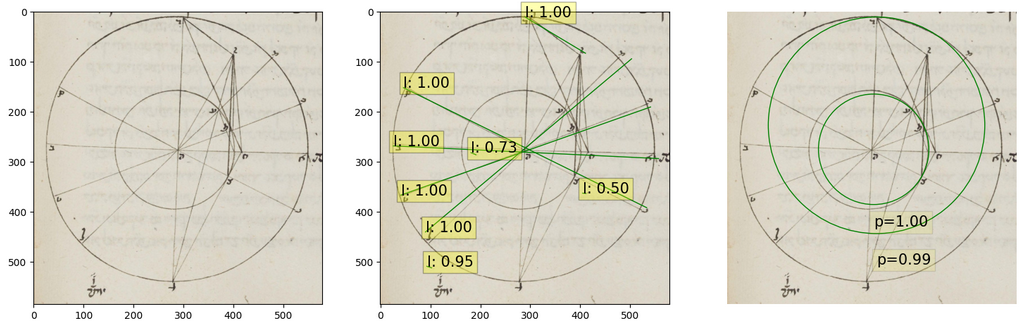
\includegraphics[width=16cm]{images/imagine_vector1.png}
		\end{subfigure}
		\hspace{1pt}
		\begin{subfigure}{1\linewidth}
			\centering
			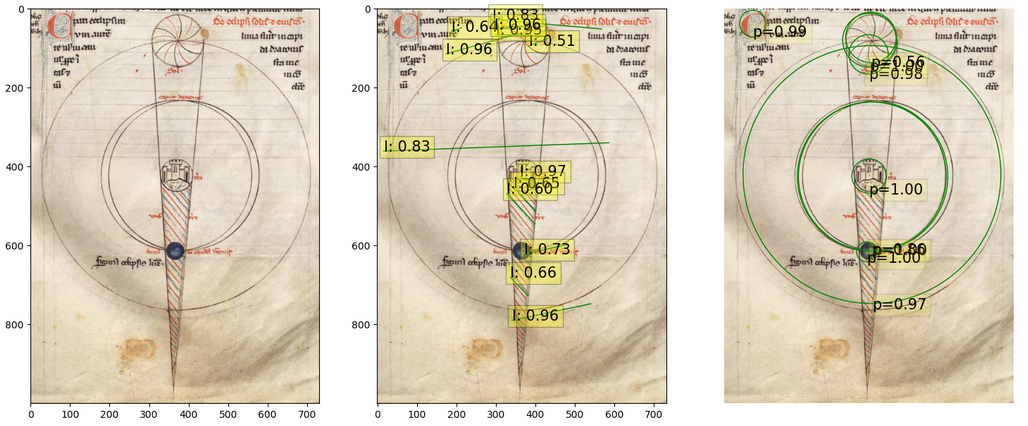
\includegraphics[width=16cm]{images/imagine_vector2.png}
		\end{subfigure}
		\caption{Résultats préliminaires de la \textit{pipeline} automatique de vectorisation sur les données du projet \eida}
		\label{fig:imagine_vector}
	\end{figure}

	\subsubsection{Intégrer la vectorisation à une chaîne de traitement automatique}
	La \textit{pipeline} automatique de vectorisation décrite peut exister dans le contexte d'une chaîne de traitement plus vaste, liée à d'autres tâches automatiques des sources pour minimiser les traitements manuels des chercheurs sur leurs documents d'étude. 
	
	Dans une chaîne de traitement telle que celle proposé par le projet \eida, la vectorisation des diagrammes intervient à la suite d'une détection automatique des objets dans les numérisations, et de la correction par les chercheurs de ce premier traitement. Ainsi, les algorithmes pour la vectorisation appliquent des traitements à des images de diagrammes qui ne comprennent plus l'ensemble d'une page numérisée, mais qui ne correspondent qu'aux limites de l'illustration détectée par le précédent algorithme. Ce premier traitement par un algorithme de détection d'objet assure la performance des algorithmes de vectorisation, tout en automatisant l'étape d'extraction des diagrammes. Entre ces deux étapes automatiques, il est préférable d'inclure une intervention manuelle, qui permet au chercheur de sélectionner les illustrations d'intérêt parmi les éléments détectés par le premier modèle, pour éviter ainsi la perte de temps que constituerait la vectorisation d'illustrations qui n'entrent pas dans le cadre du projet de recherche. 
	
	L'intégration à une plateforme d'un algorithme de détection permettant l'extraction des illustrations préalablement à la vectorisation de ces images de diagramme permet une intervention minimale du chercheur, qui sélectionne les numérisations en amont de la chaîne de traitement. Le chercheur intervient ensuite pour la correction de la détection : ainsi, la fouille dans le corpus est automatisée, permettant le traitement rapide d'un grand volume de numérisations, et la transformation des illustrations détectées puis choisies en un objet vectoriel aisément exploitable est effectuée par une suite d'algorithmes qui ne nécessite pas, pour le chercheur, de compétences techniques particulières. Cette succession permet de s'assurer du lancement de la vectorisation sur un ensemble d'images pertinent, et leur traitement automatique pour l'étape chronophage qu'est la transcription. À l'issue de ce processus, les transcriptions automatiques -- comme tout traitement par un modèle de vision artificielle -- doivent faire l'objet d'une correction, pour s'assurer de la justesse des prédictions et de la pertinence des données exploitées ou publiées.

\subsection{Données d’entraînement pour la vectorisation et correction des annotations}
    \subsubsection{Jeux de données et pratiques d'annotation}
    Pour l'entraînement et la validation d'une \textit{pipeline} de vectorisation, il est nécessaire de produire une vérité de terrain à partir d'annotations corrigées, élément indissociable de la création d'outils employant des algorithmes d'\ia. Les formats de ces jeux de données correspondent aux formats d'entrée et de sortie des algorithmes utilisés : pour la vectorisation, les données d'entrée sont des images au format PNG ou JPEG, et les prédictions sont des images vectorielles en \svg. La vérité de terrain se doit donc d'être constituée d'un ensemble de numérisations de diagrammes accompagnées d'annotations, c'est-à-dire de leur transcription en images vectorielles (fig \ref{fig:diagram_svg}).
    
    \begin{figure}[h]
    	\begin{subfigure}{0.5\linewidth}
    		\centering
    		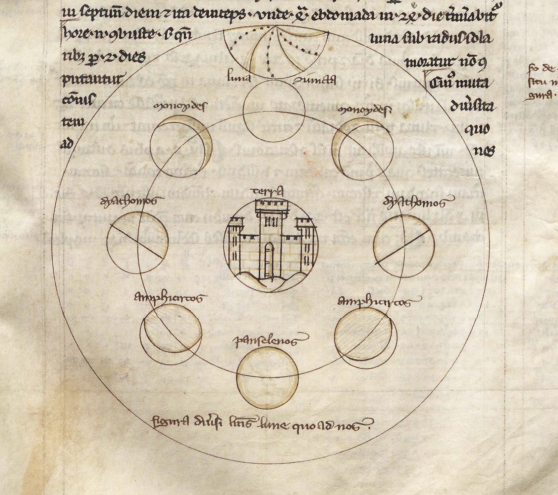
\includegraphics[width=8cm]{images/diagram8.png}
    	\end{subfigure}
    	\hspace{1pt}
    	\begin{subfigure}{0.5\linewidth}
    		\centering
    		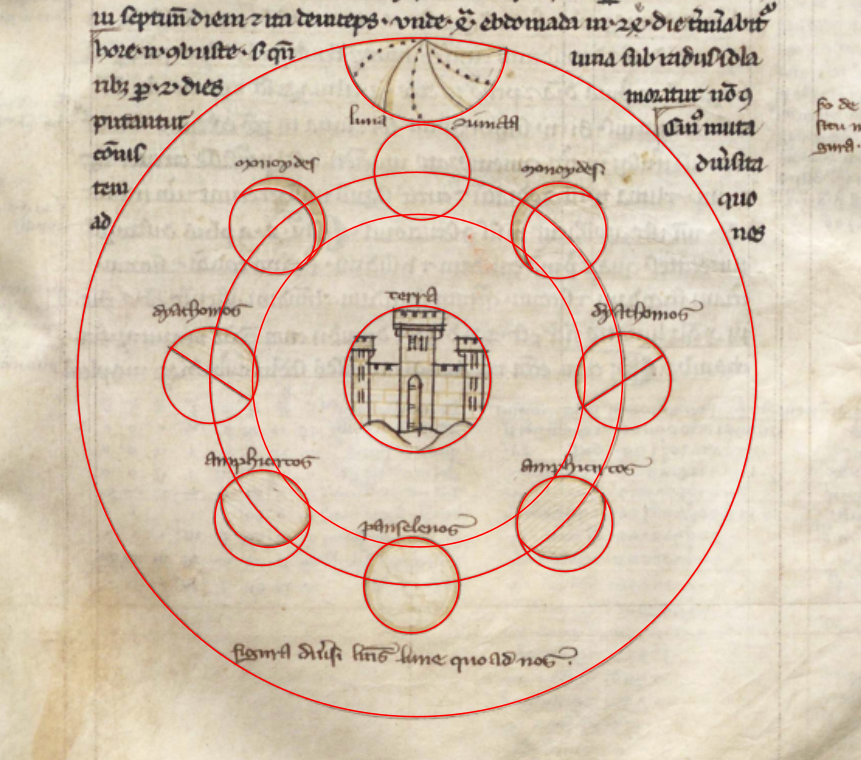
\includegraphics[width=8cm]{images/diagram8_corr.png}
    	\end{subfigure}
    	\hspace{1pt}
    	\caption{Numérisation d'un diagramme astronomique et capture d'écran de sa transcription corrigée}
    	\label{fig:diagram_svg}
    \end{figure}

	Pour la création d'une vérité de terrain, il est ainsi nécessaire d'établir des pratiques uniformes entre tous les membres d'un projet, pour s'assurer de la pertinence des résultats obtenus, basés sur ces données. Le projet \eida utilise pour la correction de ces annotations le logiciel Inkscape\footnote{Inkscape est un logiciel destiné à la création d'images vectorielles. L'utilisation du logiciel dans le projet \eida a fait l'objet d'une session de formation informelle pour la prise en main de l'outil. \cite{Inkscape}}, qui permet l'import des résultats primaires de la vectorisation pour sa correction par les chercheurs. 
	
	La méthode de vectorisation ne produisant les objets vectoriels de sortie qu'avec des cercles et des lignes, l'annotation a ainsi fait l'objet de discussions pour établir, en fonction de ces limites de la technique, les décisions scientifiques les plus pertinentes. À titre d'exemples, il est décidé que les cercles dont le tracé manuscrit est hésitant dans la source ne font l'objet que d'un unique cercle dans la version vectorielle. De même, la méthode de vectorisation ne prend pas en compte les arcs de cercle, qu'elle transcrit comme des cercles complets. Il a été décidé, après discussion, que ces arcs doivent être annotés comme des courbes et non des cercles complets, dans l'espoir d'entraîner le modèle à ce tracé spécifique. Comme pour la détection, les sources présentent de nombreux cas limites : les manuscrits d'astronomie peuvent contenir, notamment, des dessins d'astrolabe, qui dans leur forme présentent des similarités avec les diagrammes et sont d'intérêt d'un point de vue scientifique, mais qui, de par leur complexité, ne peuvent être transcrits par le modèle. Les ateliers d'annotation menés permettent ainsi d'établir un pont entre les attentes scientifiques et les possibilités techniques, prometteuses mais encore limitées, des méthodes de vectorisation automatique\footnote{Pour assurer l'uniformité des données d'entraînement d'\eida, un document de spécifications a été rédigé par les ingénieurs du projet.}. En considérant qu'un modèle de vision artificielle, même entraîné, n'est jamais aussi précis qu'un annotateur humain\footnote{Les annotations produites par un annotateur humain présentent cependant également le défaut d'être inconstantes, et cette inconstance est d'autant plus importante dans un projet impliquant plusieurs annotateurs.}, et que les transcriptions comporteront toujours des erreurs, les décisions sont prises pour l'obtention d'un modèle de vectorisation maximaliste, qui génère des faux positifs plutôt que des faux négatifs\footnote{Cette décision découle d'un constat pratique : lors de la correction des annotations, il est plus aisé de supprimer des éléments que d'en ajouter. Ce constat est valable pour la vectorisation, mais aussi pour la détection d'objets, ou pour les tâches décrites dans le chapitre suivant.}.

    \subsubsection{Une interface pour l'annotation ?}
    Un projet souhaitant avoir recours à la vision artificielle pour la vectorisation automatique d'illustrations se doit de prendre en compte la nécessité d'une interface pour la correction des annotations. Pour assurer la production de données fiables et pertinentes, une intervention manuelle par un annotateur capable de porter un regard critique sur les résultats produits est nécessaire. Dans le cadre du développement d'une plateforme à destination des chercheurs, qui intègre de tels algorithmes, il est donc nécessaire de concevoir une interface destinée à cette correction, qui permet d'intégrer cette étape à une chaîne de traitement globale, et d'éviter aux chercheurs le recours à un logiciel tiers. En prenant en considération ces besoins, \eida prévoit le développement d'une interface intégrant l'application GeoGebra pour le traitement manuel des vectorisations\footnote{Cette fonctionnalité constitue une étape future du développement de l'application \eida, le cahier des charges de l'interface n'a, à ce jour, pas été établi. Les solutions proposées sont donc abstraites ; il a cependant été constaté que GeoGebra est un outil relativement connu par les chercheurs du projet.}. Cette interface future, intégrant le modèle développé par le laboratoire \imagine, vise ainsi à accélérer le travail d'édition des diagrammes astronomiques en minimisant le temps dédié à la transcription, et à proposer un outil libre, à la prise en main aisée, à destination des chercheurs.